\begin{figure}[h]
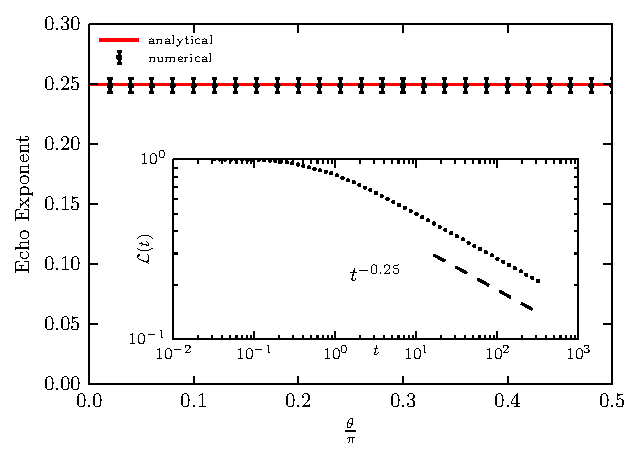
\includegraphics[width=1\columnwidth]{DDDD_fit.pdf}
\caption{The Loschmidt echo decay exponent of the process in $\text{DD}\rightarrow \lambda$ {\iffalse \color{red}Eq.~\eqref{eq:DDDD}\fi}, with gluing condition $S_1(\theta)$. We work with the total system size $N = 30000$ sites, and parameters $m = 10^{-8}$, $k = 1$. The lattice constant is set to unity. The blue dots representing the numerical results lie on the red analytic line. As predicted, the echo exponents are all equal for different values of $\theta$. Inset: An example of Loschmidt echo with $\theta = 0.02 \pi$ shown in log-log scale. The dashline denotes the expected power law of $t^{-0.25}$. Finite size effect does not emerge before $t=10^{3}$, which sets the right boundary of the range we fit. See main text for the curve fitting method.}
\label{fig:DDDD}
\end{figure}

We use the lattice model introduced in Sec.~\ref{sec_sub:free_boson_lattice} to check the analytic results. Our numerical evaluations is based on a boson Bogoliubov transformation and the explicit form of the groundstates. The readers are referred to App.~\ref{app:comp_fid_echo} for the technical details. In all the figures, we present the coefficients of the logarithmic term $\frac{\mathcal{F}}{\ln L}$ and $\frac{\mathcal{F} }{\ln t}$ and call them fidelity and echo exponents respectively. 

We first consider the process ${\rm DD} \rightarrow \lambda$
%in Eq.~\eqref{eq:DDDD}
%\begin{equation}
%\text{DD}+\text{DD}\rightarrow\lambda+\text{DD},
%\end{equation}
and show its Loschmidt echo of system size 30000 sites in Fig.~\ref{fig:DDDD}. The inset is a typical Loschmidt echo diagram, whose linearly decreasing behavior in the log-log scale indicates the expected power law decay. We also provide the analytic prediction $\mathcal{L}(t)\sim t^{-0.25}$ (\cf Eq.~\eqref{eq:result_DDDD}) as contrast. The exponent (negative of the slope of the line in log-log plot) is calculated by fitting such diagrams for $\theta = 0.01n \pi$, $n = 1,...,50 $. The fitting is performed before the finite size revival surges and error is estimated by assuming independent and identical Gaussian distribution for each point. We see that the exponents all match with the $\frac{1}{4}$ theoretical line within error. 

We also calculated the companion process ${\rm NN} \rightarrow \lambda$ and obtain identical exponents as in Fig.~\ref{fig:DDDD}. We avoid the technical subtlety of zero mode by adding a small mass regulator $m=10^{-8}$. While the short time decay pattern is different from the DD case, the long-time behavior and exponents remain the same for both echo and fidelity. We therefore do not present the result here. 

Next, we analyze the more interesting $\theta$ dependent process ${\rm DN} \rightarrow \lambda$
%in Eq.~\eqref{eq:DNDN}
%\begin{equation}
%  \text{DN}+\text{DN}\rightarrow\lambda+\text{DN},
%\end{equation}
in which the joining boundary condition is determined by $S_1(\theta)$. We worked with a system containing $35000$ sites. A direct calculation with the mass regulator do not perform very well in the small $\theta$ regime: the exponent is slightly larger than the theoretical prediction. We therefore turn to another regulator that shift the far end boundary condition DN to $S_1( \delta \theta )$ and consider the following process
\begin{eqnarray}\begin{aligned}
\label{eq:approx_DNDN}
S_1(0)+S_1(\delta\theta)\rightarrow S_1(\theta)+S_1(\delta\theta),
\end{aligned}\end{eqnarray}
\rev{ where we have used the full notation as in Eq.~\eqref{eq:Full_notation_rand()}. }
Since ${\rm DN} = S_1 (0 )$, taking smaller and smaller $\delta \theta$ should correspond to the original process. This ``shift" regulator works very well for the fidelity calculation, where $\delta \theta = 0.001 \pi$, while moderately good for the Loschmidt echo, where $\delta \theta = 0.003\pi$, see Fig.~\ref{fig:DDNN}. The inset shows the $\theta$-dependence of power law decay, and the corresponding exponents follows the quadratic relation as predicted in Eq.~\eqref{eq:result_DNDN}. %We leave further discussion of introducing $\delta\theta$ in Sec.~\ref{sec:disc}. 

\begin{figure}
  \centering
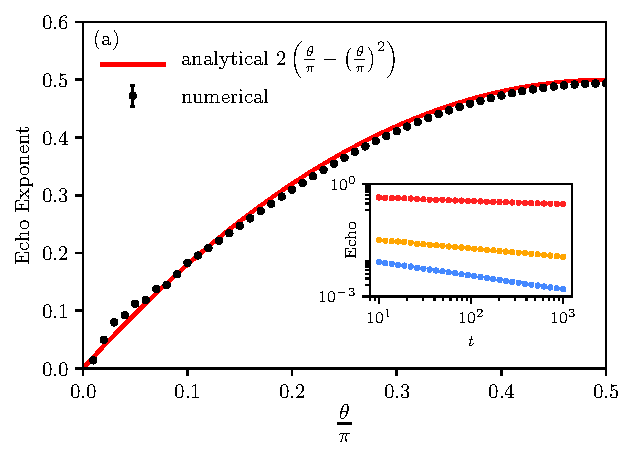
\includegraphics[width=1\columnwidth]{DDNN_fit.pdf}
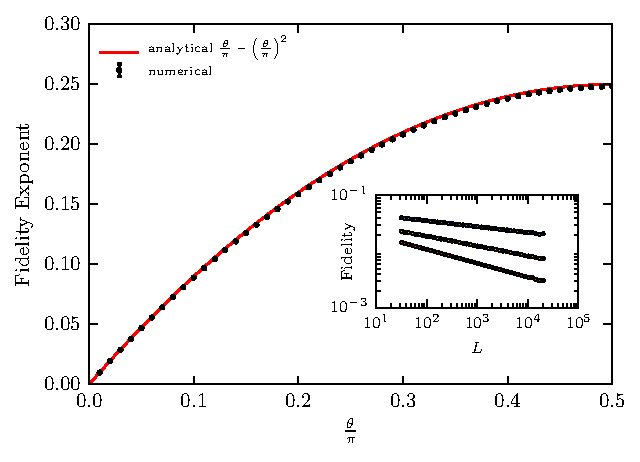
\includegraphics[width=1\columnwidth]{DDNN_fidel_fit.pdf}
    \caption{The slope of the free energy for Loschmidt echo (a) and bipartite fidelity (b) for the process $\text{DN} \rightarrow \lambda$ {\iffalse in Eq.~\eqref{eq:DNDN}\fi}. The total system size is $N=35000$ sites with the same parameters as in Fig.~\ref{fig:DDDD}. The numerical value of exponents follow a quadratic relation as predicted. There is still visible deviation from the analytic results in (a) due to the subtlety of zero mode, see the discussion in the main text. Inset in (a): From the top to bottom, we show the power law decay of Loschmidt echo with $\theta=0.02\pi, 0.12\pi $ and $0.24\pi$. Finite size effect does not emerge before $t=10^{4}$. We use the same curve fitting method as described for Fig.~\ref{fig:DDDD}.}
      \label{fig:DDNN}
\end{figure}

We finally consider the process $\text{P} \rightarrow \lambda$
% in Eq.~\eqref{eq:PP}
%\begin{equation}
%\text{P}+\text{P}\rightarrow\lambda+\text{P},
%\end{equation}
in Fig.~\ref{fig:PPPP}. Since ${\rm P} = S_1( \frac{\pi}{4} ) $, the zero mode now occurs at $\theta = \frac{\pi}{4}$. We therefore apply the shift regulator there 
\begin{equation}
\begin{aligned}
\label{eq:approx_PPPP}
S_2\left(\frac{\pi}{4}\right)+S_2\left(\frac{\pi}{4}+\delta\theta\right)\rightarrow S_2(\theta)+S_2\left(\frac{\pi}{4}+\delta\theta\right),
\end{aligned}
\end{equation}
where $\delta\theta=0.003\pi$. The $\theta$ dependent exponents are now symmetric about $\theta=\frac{\pi}{4}$ and quadratic on each side, in accordance to Eq.~\eqref{eq:periodic-case}.

\begin{figure}
  \centering
  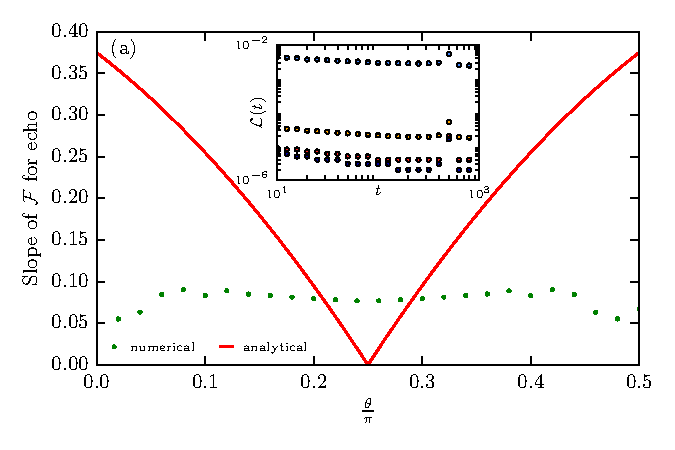
\includegraphics[width=1\columnwidth]{PP_fit.pdf}
    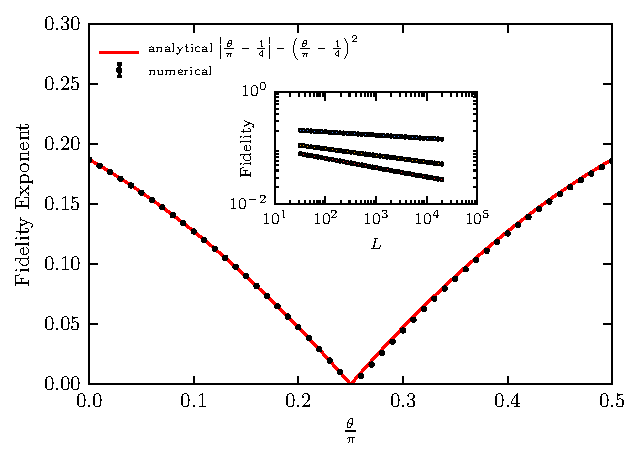
\includegraphics[width=1\columnwidth]{PP_fidel_fit.pdf}
    \caption{The decay exponent of Loschmidt echo (a) and bipartite fidelity (b) for the process $\text{P} \rightarrow \lambda${\iffalse in Eq.~\eqref{eq:PP}\fi}. The parameters are the same as those in Fig.~\ref{fig:DDNN}. The plot is symmetric with respect to $\theta=0.25\pi$ as predicted. The deviation around $\frac{\pi}{4}$ in (a) is small but visible, see the discussion in the main text. Inset in (a): From top to bottom, we show the power law decay of Loschmidt echo with $\theta=0.04\pi, 0.08\pi $ and $0.18\pi$. Finite size effect does not emerge before $t=10^{4}$. We use the same curve fitting method as described for Fig.~\ref{fig:DDDD}.}
    \label{fig:PPPP}
\end{figure}

Finally, we also provide the data for the process
\begin{equation}
\label{eq:DNP_rand()}
{\rm DN} + {\rm P} \rightarrow \lambda  + {\rm P},
\end{equation}
to evaluate the influence of the boundary condition $c$. It {\rm does} influence the scaling dimension, which is not captured by our analytic calculation. We note that the exponent still follows the quadratic relation with a deficit of $\frac{1}{8}$ at large value of $\theta$. The deficit approaches zero at $\theta=0$ where the setups are the same before and after quench.
\begin{figure}[htb]
\centering
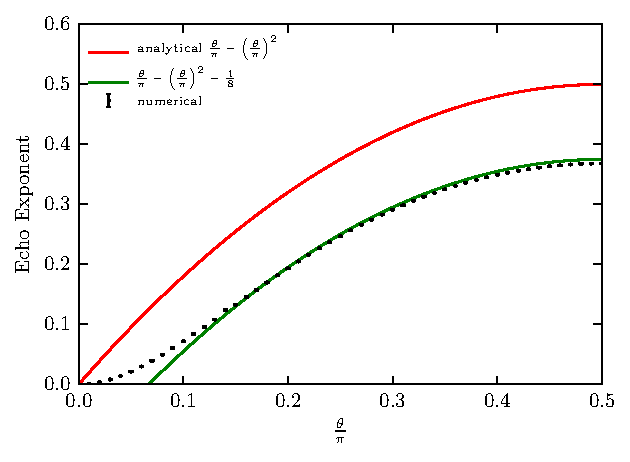
\includegraphics[width=1\columnwidth]{PDN_fit.pdf}
\caption{The decay exponent of Loschmidt echo for the process {\color{red}in Eq.~\eqref{eq:DNP_rand()}.} The boundary condition $c$, which is now different from $a$, changes the scaling completely from the analytic quadratic curve. The deficit to the analytic value is roughly $\frac{1}{8}$ for $\theta > \frac{\pi}{4}$, It becomes smaller and approaches zero for small $\theta$. }
\label{fig:PDN_fit}
\end{figure}

%%% Local Variables:
%%% TeX-master: "bCFT_paper"
%%% TeX-PDF-mode: t
%%% End:
